%% ****** Start of file apstemplate.tex ****** %
%%
%%
%%   This file is part of the APS files in the REVTeX 4 distribution.
%%   Version 4.1r of REVTeX, August 2010
%%
%%
%%   Copyright (c) 2001, 2009, 2010 The American Physical Society.
%%
%%   See the REVTeX 4 README file for restrictions and more information.
%%
%
% This is a template for producing manuscripts for use with REVTEX 4.0
% Copy this file to another name and then work on that file.
% That way, you always have this original template file to use.
%
% Group addresses by affiliation; use superscriptaddress for long
% author lists, or if there are many overlapping affiliations.
% For Phys. Rev. appearance, change preprint to twocolumn.
% Choose pra, prb, prc, prd, pre, prl, prstab, prstper, or rmp for journal
%  Add 'draft' option to mark overfull boxes with black boxes
%  Add 'showpacs' option to make PACS codes appear
%  Add 'showkeys' option to make keywords appear
\documentclass[footinbib,aps,prl,twocolumn,superscriptaddress]{revtex4-1}
%\documentclass[aps,prl,preprint,superscriptaddress]{revtex4-1}
%\documentclass[aps,prl,reprint,groupedaddress]{revtex4-1}

% You should use BibTeX and apsrev.bst for references
% Choosing a journal automatically selects the correct APS
% BibTeX style file (bst file), so only uncomment the line
% below if necessary.
%\bibliographystyle{apsrev4-1}

\usepackage{amsmath}
\usepackage{graphicx}
\graphicspath{{../Graphics/}}
\usepackage{gensymb}


\begin{document}

% Use the \preprint command to place your local institutional report
% number in the upper righthand corner of the title page in preprint mode.
% Multiple \preprint commands are allowed.
% Use the 'preprintnumbers' class option to override journal defaults
% to display numbers if necessary
%\preprint{}

%Title of paper
\title{Polarization state generation and measurement in parallel with a single metasurface}

% repeat the \author .. \affiliation  etc. as needed
% \email, \thanks, \homepage, \altaffiliation all apply to the current
% author. Explanatory text should go in the []'s, actual e-mail
% address or url should go in the {}'s for \email and \homepage.
% Please use the appropriate macro foreach each type of information

% \affiliation command applies to all authors since the last
% \affiliation command. The \affiliation command should follow the
% other information
% \affiliation can be followed by \email, \homepage, \thanks as well.
%\author{Noah A. Rubin}
%\author{Federico Capasso}
%\email[]{capasso@seas.harvard.edu}
%\homepage[]{Your web page}
%\thanks{}
%\altaffiliation{}
%\affiliation{John A. Paulson School of Engineering and Applied Sciences, Harvard University, Cambridge, MA 02138, USA}

%Collaboration name if desired (requires use of superscriptaddress
%option in \documentclass). \noaffiliation is required (may also be
%used with the \author command).
%\collaboration can be followed by \email, \homepage, \thanks as well.
%\collaboration{}
%\noaffiliation

\date{\today}

\begin{abstract}
The constituent elements of metasurfaces may be designed with explicit polarization-dependence, making metasurfaces a fascinating platform for new polarization optics. In this work we show that, using a simple optimization scheme, a metasurface grating can be designed producing arbitrarily specified polarization states on a set of defined diffraction orders given that the polarization of the incident beam is known. We also demonstrate that, used in a reverse configuration, the same grating may be used as a parallel snapshot polarimeter, requiring a minimum of bulk polarization optics. We characterize its performance and show that its accuracy matches that of a commercial rotating waveplate polarimeter.
\end{abstract}

% insert suggested PACS numbers in braces on next line
%\pacs{}
% insert suggested keywords - APS authors don't need to do this
%\keywords{}

%\maketitle must follow title, authors, abstract, \pacs, and \keywords
\maketitle

% body of paper here - Use proper section commands
% References should be done using the \cite, \ref, and \label commands
%\frame{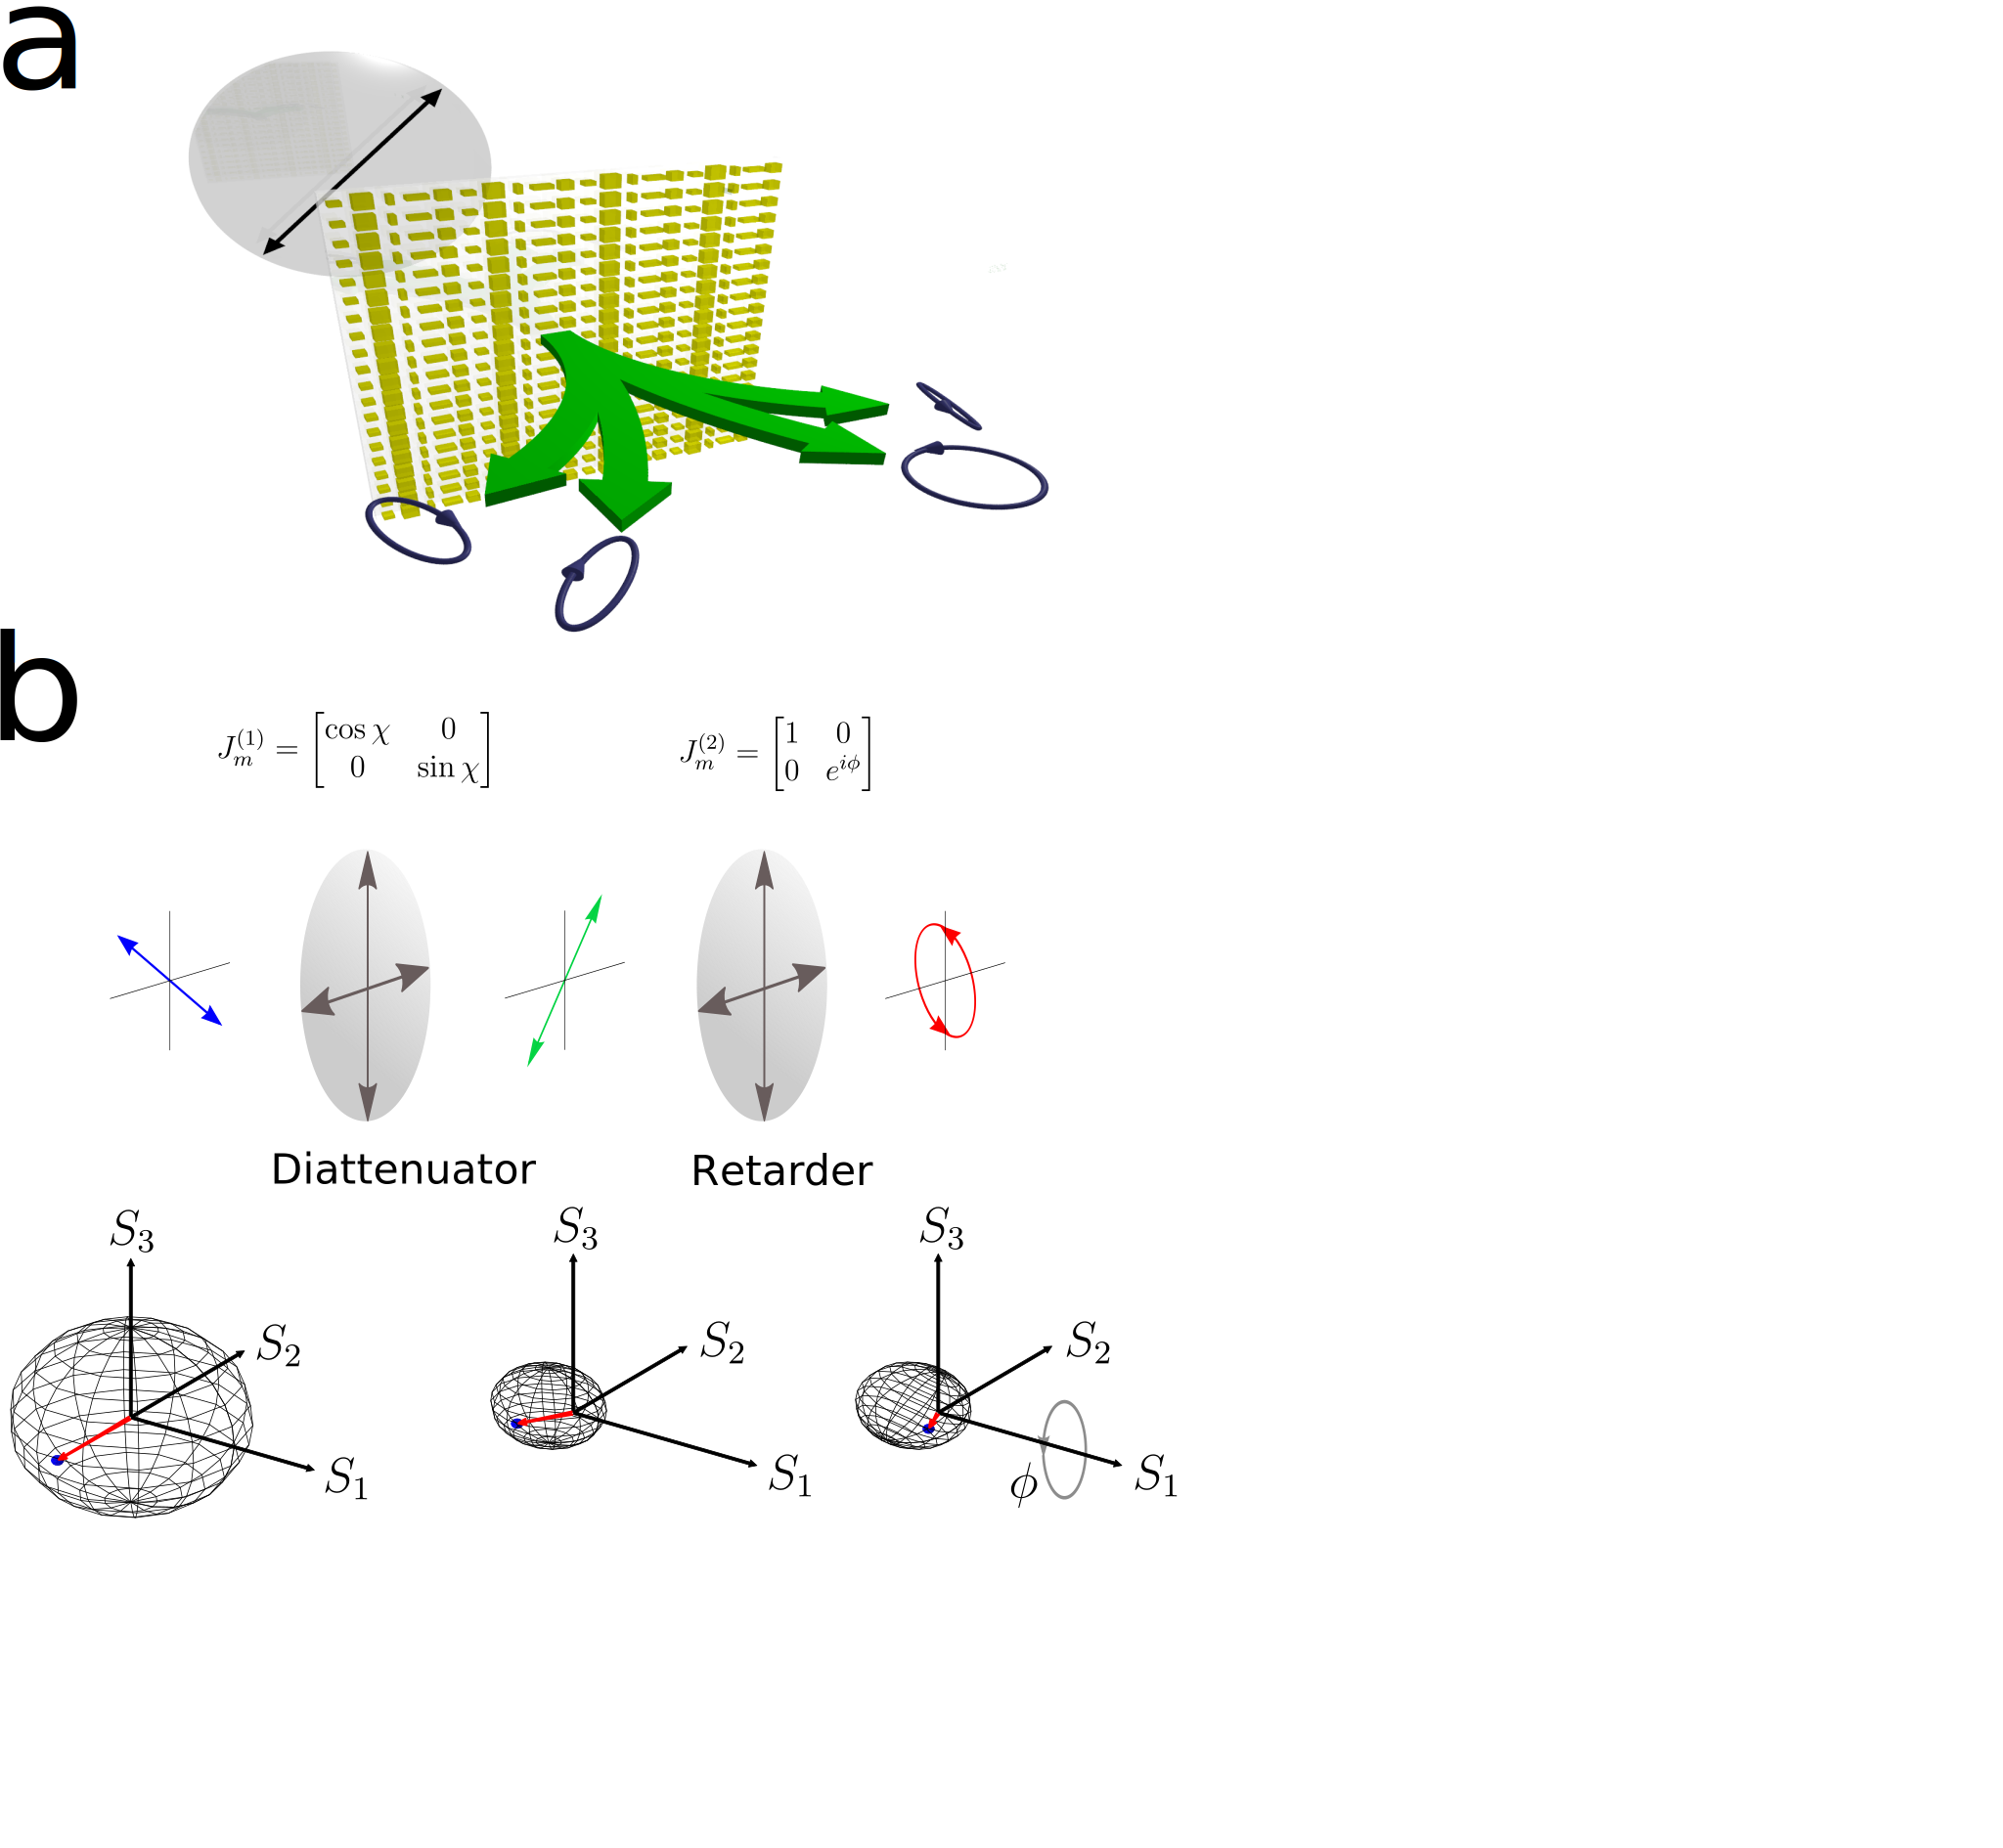
\includegraphics[width=\textwidth]{Fig1.eps}}

\begin{figure*}[!htp]
	\centering
	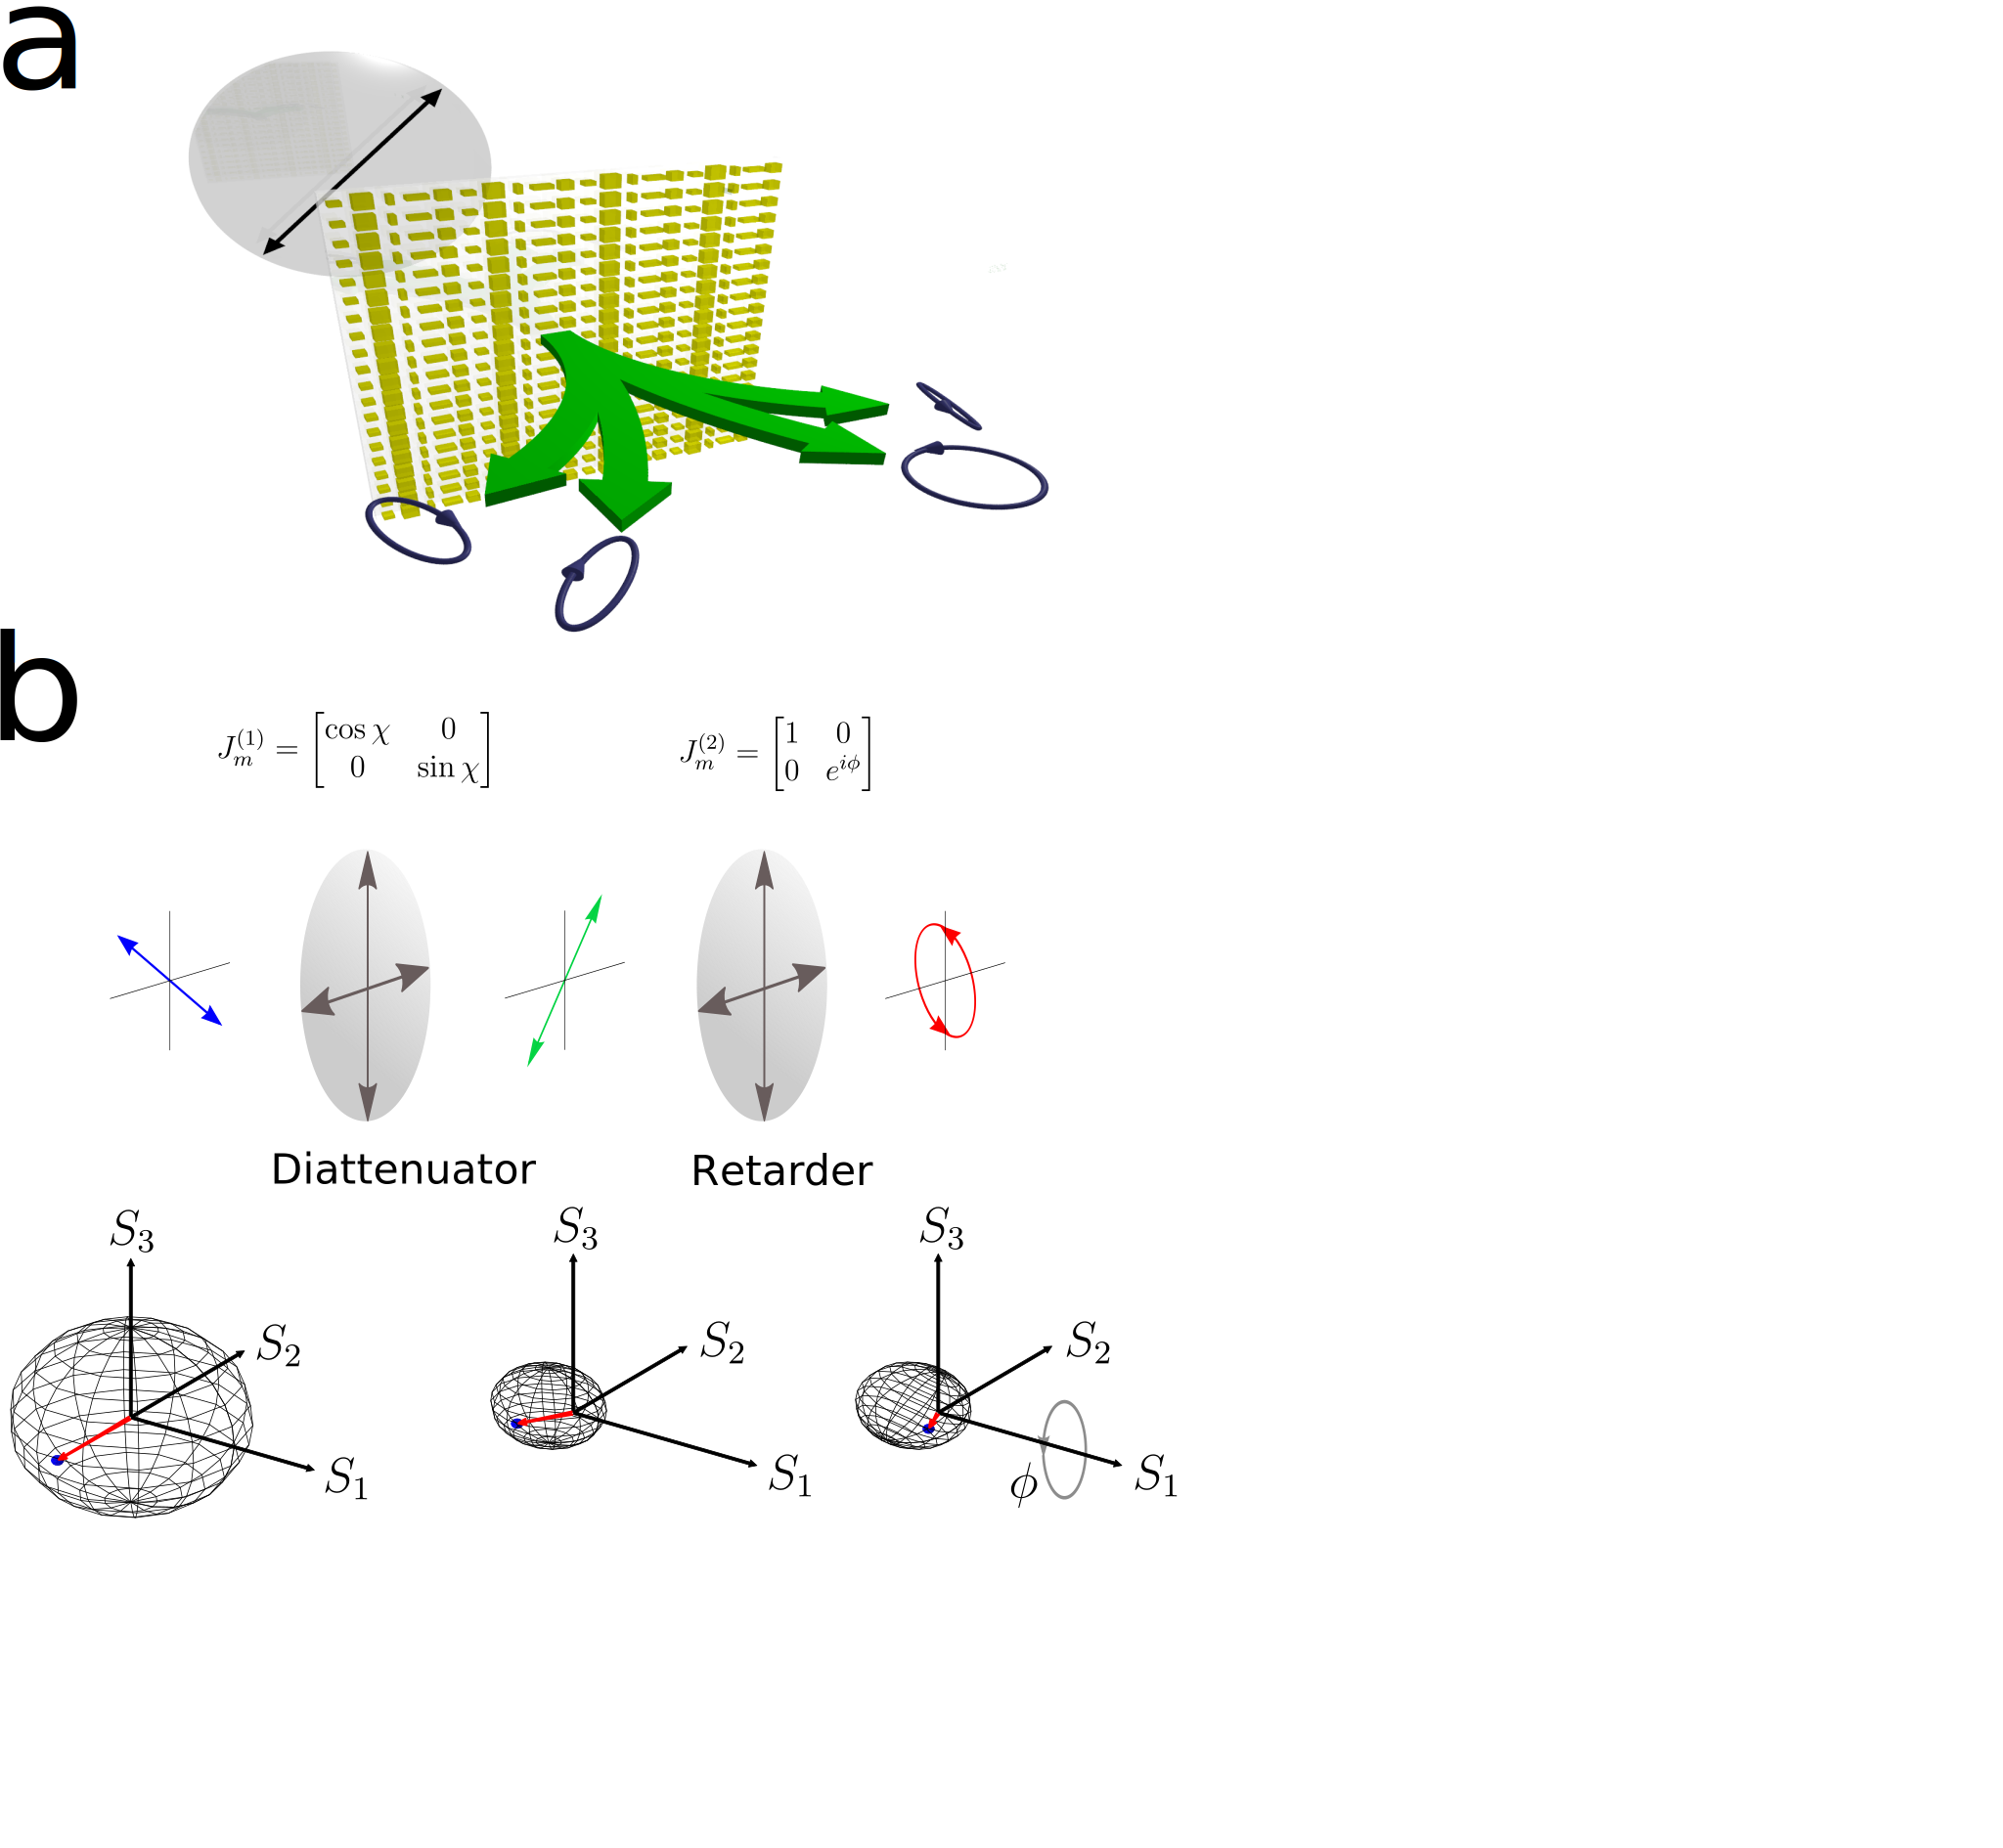
\includegraphics[width=\textwidth]{Fig1.pdf}
	\caption{\label{fig:fig1}}
\end{figure*}

\section{Introduction}

As an essential aspect of electromagnetic radiation, polarization plays a role of paramount importance in countless areas of science and technology. Aside from polarization's clear role in atomic physics, optics, and fundamental light/matter interaction \cite{Born1999a}, polarization-dependent effects are of technological significance in fiber-optic telecommunications \cite{Damask2005, Yariv2006}, while polarization-resolved imaging can highlight features that, by other means, would be rendered practically invisible \cite{Tyo2006, Snik2014}. This has found application in remote sensing \cite{Tyo2006}, aerosol characterization and atmospheric science \cite{Deschamps1994}, and even non-invasive cancer pathology and diagnosis \cite{Novikova2012, Pierangelo2013}. Polarization-resolved methods find extensive use in observational astronomy \cite{Keller2001}, in areas such as exoplanet discovery \cite{Wiktorowicz2014} and especially solar astrophysics \cite{Stenflo1994}. For these reasons and more, methods of producing, measuring, and manipulating polarized light are of significant scientific and technological interest.

The basic units of polarization optics are polarizers and phase retarders. Various polarizer technologies exist, including wire-grid, dichroic crystals, birefringent crystal prisms, and the famed sheet polarizers of E. Land and the Polaroid Corp. \cite{Damask2005, Shurcliff1962}. Phase retarders most commonly take the form of bi/unaxial crystals, the subject of the first scientific investigations into polarization optics, whose birefringent properties allow for polarization conversion. These plates are difficult to fabricate and challenging to integrate.

The generation and analysis of polarization are conjugate problems --- any polarization state generator may function as an analyzer, if used in reverse. Polarization state measurement, commonly known as polarimetry \cite{Azzam2016}, then, largely relies on the same technologies detailed above. Stokes polarimetry in particular involves the determination of the full, four-component polarization Stokes vector $\vec{S} = \begin{bmatrix} S_0 & S_1 & S_2 & S_3 \end{bmatrix}^T$, which quantifies both the parameters of the polarization ellipse but also the overall beam intensity and its degree of polarization (discussed further below). If an unknown Stokes vector $\vec{S}_{\text{inc}}$ is incident on an analyzer, a detector would observe, as a consequence of time-reversal symmetry an intensity $I_{\text{meas}} \propto  \vec{S}_{\text{inc}} \cdot \vec{S}_{c}$, where $S_c$ is the characteristic polarization produced by the analyzer, were it used as a generator. The process of polarimetry amounts to several such projective measurements of the Stokes vector. This is formalized in the equation:

\begin{equation}
	A\vec{S} = \vec{I}
\end{equation}

Here, $A$ is an $N \times 4$ matrix, $\vec{S}$ is an incident Stokes four vector, and $\vec{I}$ is a list of $N$ measured intensities. That is, the matrix $A$ (known as the instrument matrix) links the parameters of the polarization Stokes vector with measured intensity values on different analyzer channels. In the special case of $N=4$, then, we can write straightforwardly that $\vec{S} = A^{-1} \vec{I}$ (in the more general case where $N > 4$, one can solve for $\vec{S}$ in the least-squares sense). 

The measurements making up $\vec{I}$ may be performed in various ways, but several broad categories of Stokes polarimeters exist. In the so-called division-of-time approach, a detector with a single set of polarization optics is used. The optics sequentially take on $N$ configurations. Each element, or channel, in the vector $\vec{I}$ is a measurement at a given configuration. While this reduces the number of necessary optical components, ultimately the time resolution of this approach is limited by the speed at which the polarization optics may be readjusted. In the case of mechanical rotation, this represents a severe handicap. Active polarization optics such as liquid-crystal variable retarders ameliorate this issue somewhat, though here too, the resolution is limited to (approximately) the ms range, at great expense \cite{Snik2014}.

A second broad approach is division-of-amplitude (also known as parallel, or snapshot, polarimetry). In this approach, the wavefront is divided among $N$ parallel channels each of which implements a different analyzer. In traditional implementations, this may be accomplished by the use of birefringent (e.g., Wollaston) prisms and beamsplitters \cite{Azzam1982}, or by employing a diffraction grating to split the beam into $N$ channels each of which contains its own unique polarization optics and a detector \cite{Azzam1993, Cui1996}. This variety of polarimetry is desirable because the time-resolution of Stokes vector determination is limited only by the detection electronics themselves. A major drawback, however, is the need for distinct polarization optics on each channel, which increases the complexity and expense of any such system. Additionally, the bulk of these components hinders integration and widespread use.

Meanwhile, metasurfaces \cite{Yu2011} --- that is, subwavelength-spaced arrays of nanophotonic phase-shifting elements --- have emerged as a fascinating new platform for flat, diffractive optics. Among the most powerful features of metasurfaces are the sophistication with which the individual phase-shifting elements may be engineered. In particular, this allows for nano-scale elements with tunable structural birefringence; This aspect in particular makes metasurfaces a fascinating new platform for polarization optics \cite{Arbabi2015, Mueller2017}.

In this work, we present a scheme for the design of a metasurface diffraction grating that, when light of a known polarization is incident, may produce desired states of polarization in parallel on its diffraction orders. We characterize several fabricated gratings designed with this scheme. By the reciprocity discussed above, the same grating may act as a parallel full-Stokes polarimeter, notably one that requires no bulk birefringent optics. We characterize such a polarimeter, including its performance with partially/un-polarized light, and find that it compares favorably to a commercial rotating waveplate polarimeter. This work is of consequence for any application requiring low-cost, easily integrated polarimetry and is a testament to the flexibility of metasurfaces in the realm of polarization optics.

\section{Principle of Operation}

Metasurfaces, if fashioned from individual phase-shifting elements with inherent structural birefringence, can achieve wide-ranging polarization functionalities \cite{Arbabi2015, Mueller2017}. In particular, a metasurface element with two perpendicular symmetry axes \cite{Menzel2010} can function as a waveplate-like phase shifter, imparting independent phases $\phi_x$ and $\phi_y$ on $x$ and $y$ polarized light whose values may be arbitrarily tuned by adjusting the dimensions $w_x$ and $w_y$ (Fig. \ref{fig:fig1}b). If $N$ such birefringent phase shifters are arranged in a 1D  periodic unit cell (Fig. \ref{fig:fig1}c), we can denote the phase shift experienced by $x$ polarized light at the $n^{\text{th}}$ position in the unit cell by $\phi_x^n$. That is, we may approximate the phase shift acquired by the wavefront at each position in the unit cell as constant. This discrete phase profile $\phi_x(\tilde{x})$ experienced by $x$ polarized light, as a function of the spatial coordinate $\tilde{x}$ (not to be confused with $x$ polarized light), can be written as a vector, $\vec{\Phi}_x = \{\phi_x^{(1)}, ..., \phi_x^{(N)}\}$ with $\vec{\Phi}_y$ holding an analogous meaning for $y$ polarized light. If the periodic unit cell is tessellated, we form a birefringent metasurface that functions as an independent phase grating for orthogonal $x$ and $y$ polarizations, or a \textit{polarization grating}.

Being periodic, the angular spectrum is discrete. Given the phase profiles $\phi_x(\tilde{x})$ and $\phi_y(\tilde{x})$, we may compute the Fourier decomposition of each phase grating onto the $m^{\text{th}}$ grating order:

\begin{equation}
	\label{fourier_x}
	c_x^{m} = 
	\frac{1}{2\pi}\int_{0}^{d} e^{i \phi_x(\tilde{x})} e^{i \frac{2\pi m \tilde{x}}{d}} d\tilde{x}
\end{equation}

and

\begin{equation}
	\label{fourier_y}
	c_y^{m} = 
	\frac{1}{2\pi}\int_{0}^{d} e^{i \phi_y(\tilde{x})} e^{i \frac{2\pi m \tilde{x}}{d}} d\tilde{x}
\end{equation}

where $d$ is the length of the periodic unit cell and $\{c_x^m\}$ and $\{c_y^m\}$ are the Fourier coefficients of the gratings experienced by $x$ and $y$ polarizations. 

Each coefficient is complex, so we can write $c_x^m = |c_x^m| e^{i \delta_x^m}$ and $c_y^m = |c_y^m| e^{i \delta_y^m}$. Then, we can ascribe to each order a Jones matrix $J^m$:

\begin{equation}
	\label{equivalent}
	J^m = \begin{bmatrix}
			c_x^m & 0 \\ 0 & c_y^m
		  \end{bmatrix} =
		  \begin{bmatrix}
		  	|c_x^m| & 0 \\ 0 & |c_y^m|
		  \end{bmatrix}
		  \begin{bmatrix}
		  	e^{i\delta_x^m} & 0 \\ 0 & e^{i\delta_y^m}
		  \end{bmatrix}
\end{equation}

The polarization properties of order $m$ contained in $J^m$ can by seen as equivalent to a cascade of two bulk optical elements (Fig. \ref{fig:fig1}e): The first Jones matrix in the product is that of a diattenuator---that is, an imperfect polarizing element selectively attenuating light along the $x$ and $y$ directions, while the second Jones matrix is that of a phase retarder---a waveplate---with retardance $\delta^m = \delta_x^m - \delta_y^m$. Both have their eigenaxes oriented along $x$ and $y$. 

If a beam linearly polarized at $45\degree$ with electric field amplitude $E_0$ is incident on the grating, the electric field on the $m^{\text{th}}$ grating order will be:

\begin{equation}
\vec{E}^m =  E_0\begin{bmatrix} c_x^m \\ c_y^m \end{bmatrix}
\end{equation}

In the special case of $45\degree$ polarized light, then, the complex grating coefficients $\{c_x^m\}$ and $\{c_y^m\}$ directly yield the polarization state of order $m$. In a more general case, the output polarization state can be understood with aid of the Poincar\'e sphere (Fig. \ref{fig:fig1}f). All possible incident polarization states can be represented on the normal Poincar\'e sphere (a). The effect of a diattenuator is a deformation of the original sphere along the $\pm S_1$ axis (b). Then, the deformed sphere is rotated around the $S_1$ axis by an angle of $\delta^m$ representing the effect of the retarder (c); the resulting sphere represents the output polarization state on order $m$ as a function of input polarization state \cite{Damask2005}.

\section{Optimization}
% Put \label in argument of \section for cross-referencing
%\section{\label{}}

For a grating with given $\vec{\Phi}_x$ and $\vec{\Phi}_y$ and an incident beam of known polarization, then, the polarization state and power on each diffraction order $m$ can be computed with simple Fourier optics. Is it possible to deduce what $\vec{\Phi}_x$ and $\vec{\Phi}_y$ produce diffraction orders with specified states of polarization for a given incident polarization? This functionality would ordinarily require a diffraction grating with at least $2N$ waveplates, where $N$ is the number of diffraction orders to be controlled; if the required $\vec{\Phi}_x$ and $\vec{\Phi}_y$ are known, this functionality could be integrated into a single metasurface (Fig. \ref{fig:fig1}d).

Suppose a desired polarization is specified for a set of diffraction orders $q$. These polarization states dictate $\{c_x^m\}$ and $\{c_y^m\}$, the Fourier coefficients. The requisite grating could be found by simply inverting the Fourier transform. In the case of incident light polarized at $45\degree$, the required holographic mask is given by:

\begin{equation}
\label{holographic}
	\sum_{m \in q} \Big(c_x^m \begin{bmatrix}
	1 \\ 0
	\end{bmatrix} + c_y^m \begin{bmatrix}
	0 \\ 1
	\end{bmatrix}\Big) e^{-i \frac{2\pi m \tilde{x}}{d}}
\end{equation}

However, Eq. \ref{holographic}, being the sum of many spatial harmonics of the grating, requires both amplitude and phase modulation. In the realm of metasurfaces, this is undesirable. In designing constituent elements for metasurfaces, the goal is generally to obtain a range of parameter dimensions with nearly uniform amplitude transmission that yield phase shifts ranging between $0$ and $2\pi$. It is generally difficult---at least, with a limited set of possible geometries of simple design---to assemble a library of structures yielding arbitrarily shape-tunable phase shift and transmission simultaneously. In the present case, we would require that this be achievable for both $x$ and $y$ polarizations as well, independent of one another. This is, without resorting to a very large range of simulated geometries, untenable.

We desire, then, a phase-only grating. Since the exact solution (Eq. \ref{holographic}) is in general \textit{not} a phase-only grating, we must turn to optimization. In the present case, we wish to design a grating that, when light linearly polarized at $45\degree$ is incident, produces desired polarization states on a set of grating orders $\{q\}$. The desired Jones vector on each order $m \in \{q\}$ is given by

\begin{equation}
	\vec{j}^m = 
	\begin{bmatrix}
	\cos\chi^m \\ \sin\chi^m e^{i\phi^m}
	\end{bmatrix}
\end{equation}

Since a phase-only solution is not exact, light will generally be directed into all diffraction orders, not just those in $\{q\}$. However, we wish to direct as much of the incident power as possible into the desired orders. That is, we wish to maximize

\begin{equation}
	\label{merit}
	\eta(\vec{\Phi}_x, \vec{\Phi}_y) = \sum_{m \in \{q\}} \sqrt{\Big(c_x^m(\vec{\Phi}_x)\Big)^2 + \Big(c_y^m(\vec{\Phi}_y)\Big)^2}
\end{equation}

under the constraints:

\begin{equation}
	\label{pol_constraint_1}
	\frac{\lvert c_y^m \rvert}{\lvert c_x^m \rvert} = \tan \chi^m
\end{equation}

and

\begin{equation}
	\label{pol_constraint_2}
	\delta_x^m - \delta_y^m = \phi^m
\end{equation}

The vectors $\vec{\Phi}_x$ and $\vec{\Phi}_y$ are the quantities to be optimized---if the grating has $N$ constituent elements, then the optimization will involve $2N$ parameters. $N$ and the inter-element separation dictate the grating period $d$ which, along with the operating wavelength $\lambda$, specifies the angular separation of the grating orders. Once optimized $\vec{\Phi}_x$ and $\vec{\Phi}_y$ are obtained, the power in the desired orders and correspondence with the desired polarization can be directly examined (cf. Eqns. \ref{merit}, \ref{pol_constraint_1}, and \ref{pol_constraint_2}).

In this work, we perform a simple gradient descent optimization of $\eta(\vec{\Phi}_x, \vec{\Phi}_y)$ under the above constraints, with randomly generated initial conditions. This procedure alone, at least mathematically, yields high efficiencies while nearly exactly satisfying the constraints. For reasons detailed in the supplement, these optimized phase profiles, when converted to a set of geometries $w_x$ and $w_y$, perform poorly in FDTD simulation. Instead, the optimized $\vec{\Phi}_x$ and $\vec{\Phi}_y$ from gradient descent are used as the initial conditions to a gradient-free optimization of Eq. \ref{merit} which explicitly considers the simulated properties of the elements in the available library of structures.

Using this simple optimization strategy, we design two such gratings, both designed to operate at $\lambda = 532$ nm, but we stress that nothing fundamental about this work is specific to this wavelength. For each element in the optimized $\vec{\Phi}_x$ and $\vec{\Phi}_y$, a rectangular TiO$_2$ pillar is selected from a library which best imparts the required phase on $x$ and $y$ polarized light. The designed gratings are then fabricated on a glass substrate with a process extensively detailed elsewhere \cite{Devlin2016a}.

The first grating is designed to produce $+45\degree$ linear, right-circular, left-circular, and $-45\degree$ linear polarizations on the $m = -2$, $-1$, $+1$, and $+2$ diffraction orders, respectively, all with equalized intensities, when $45\degree$ linear polarized light is incident. These represent a set of polarizations commonly used in optics experiments.

The second grating is designed to produce four polarization states corresponding to the vertices of a tetrahedron inscribed in the Poincar\'e sphere on the $m = -2$, $-1$, $+1$, and $+2$ orders, all with equalized intensities, when $45
\degree$ linear polarized light is incident. This set of polarizations is of significance in polarimetry, where it represents an optimal sampling set for four-state polarimeters (discussed below) \cite{Sabatke2000, Tyo2002}.

In both cases, the gratings contained $N = 20$ individual elements, so each optimization involved $2N = 40$ parameters. This $N$ was found, heuristically, to produce results that achieve both high efficiency and correspondence with the desired polarization ellipses --- both mathematically and from FDTD simulation of the obtained geometries --- while minimizing the number of parameters to be optimized.

For each grating, the optimized phase profiles $\vec{\Phi}_x$ and $\vec{\Phi}_y$ and a schematic of the corresponding geometries implementing these phase shifts are shown in Fig. 2. Each such unit cell was tessellated into bulk metasurface gratings each $250 \times 250$ $\mu$m in size, of which SEMs are also shown in Fig. 2.

\section{Polarization State Generation}

As described above, each grating was designed to produce the desired polarization states for incident light linearly polarized at $45\degree$. A simple experiment was constructed in which each metasurface grating was illuminated with laser light of this polarization at $\lambda=532$ nm. The polarization state of the light on each of the diffraction orders of interest was then measured with a commercial rotating waveplate polarimeter (further details about this measurement are deferred to the supplement).

In Fig. 2, for each grating, the measured polarization ellipses for each order are plotted alongside the desired, designed ellipses as well as the ellipses predicted by Fourier transform of the phase profiles and an FDTD simulation of the grating. On a qualitative level, it can be seen that the polarization states produced by the fabricated gratings compellingly approximate the desired ellipses, confirming the success of the optimization scheme.

More specifically, 

...

These results are presented in Table 1.

\section{Metasurface Polarimetry}

\begin{figure*}[!htp]
	\centering
	\includegraphics[width=\textwidth]{Fig3.pdf}
	\caption{\label{fig:fig3}}
\end{figure*}

Each order of the metasurface polarization grating can be thought of as a diattenuator in series with a phase retarder, both oriented along $x$/$y$ (Eqn. \ref{equivalent}). When light from a source passes through a polarizer oriented at $45\degree$, a polarization state is produced on the grating order, ideally close to some design state (Fig. \ref{fig:fig3}a, top). As described in the Introduction, when the grating is used in a reverse configuration --- that is, with the grating followed by a linear polarizer oriented at $45\degree$ --- each diffraction order may be thought of as a polarization state analyzer for its characteristic Stokes vector (Fig. \ref{fig:fig3}a, bottom).


Given this, the grating itself may be used as a parallel full-Stokes polarimeter with no polarization optics (with the exception of a single polarizer, which may be easily integrated on top of the grating --- the polarizer is indeed necessary for determining the Stokes vector, a point we take up in the supplement). This of course relies on a suitable choice of analyzer states. The first grating presented above, producing a set of orthogonal linear states and the two circular polarizations, is not sufficient for full-Stokes polarimetry. For a polarimeter making $N=4$ measurements, it has been extensively documented in the literature that, at least in the absence of calibration errors \cite{Tyo2002}, a configuration of analyzers whose characteristic Stokes vectors correspond to (any) tetrahedron inscribed in the Poincar\'e sphere yields maximum signal-to-noise ratio in Stokes vector determination \cite{Sabatke2000}.

In acknowledgment of this fact, a larger version (1.5 mm $\times$ 1.5 mm) of the tetrahedron grating described above was fabricated. The grating is placed in a custom mount; when laser light is incident, the four diffraction orders of interest pass through a polarizer oriented at $45\degree$ and diverge. Some distance away (cms.), each beam impinges on a standard silicon photodiode, producing a photocurrent which is amplified and converted to digital form (Fig. \ref{fig:fig3}c, right side). Each measured voltage is proportional to the intensity present at the photodiode.

\subsection{Calibration}

The performance of any polarimeter relies on accurate calibration. Calibration is, essentially, the process of determining the instrument matrix $A$; the simplest possible form of calibration involves exposing the polarimeter to beams of at least four known polarization states (which themselves are independent). If the intensities on the channels of interest are recorded in response to these calibration states, the instrument matrix can be straightforwardly determined  \cite{Azzam2016}.

The accuracy of any Stokes polarimeter depends on the degree of accuracy with which these polarization states are known. Accordingly, we use a calibration scheme \cite{Azzam1989} developed for the well-known four-detector photopolarimeter of Azzam \cite{Azzam1985}, applicable to any polarimeter with four intensity channels ($N=4$). In particular, the scheme explicitly accounts for imperfect quarterwave-plates, so long as their deviation from $90\degree$ retardance is a small angle.

The first step of the calibration involves exposing the polarimeter to a large set of linear polarization states (Fig. \ref{fig:fig3}c, with the omission of boxed components (i) and (ii)). As the linear polarizer is rotated, the intensity of the beam varies due to the laser having a preferred polarization state. To account for this, at each linear polarization angle, the total beam intensity is measured by a photodiode that moves in and out of the incident beam as part of an automated measurement procedure. The photodiode is placed directly in the beam to avoid any polarization-dependence manifest in reflection from, e.g., a beamsplitter, which would destroy the integrity of the calibration.

For each linear polarization angle $\theta$, the intensity on each channel can be normalized by the incident intensity and plotted, producing four trigonometric curves. The fitting parameters of the four curves yield the first three columns of the $4\times4$ instrument matrix \cite{Azzam1989}. The last column is obtained by use of a linear polarizer and quarterwave-plate in tandem (Fig. \ref{fig:fig3}c, including boxed component (ii) and omitting (i)). This is described in the supplement.

Based on data from the calibration, each entry of the resultant instrument matrix $A$ may be assigned error bounds. These error bounds may be used to directly compute the full covariance matrix of any computed Stokes vector \cite{AsensioRamos2008}, allowing us to place error bars on any Stokes vector predicted by the metasurface grating polarimeter.

\subsection{Quantifying Partially Polarized Light}

With the metasurface grating polarimeter thus calibrated, the Stokes vector of any incident beam may be determined. An interesting case is that of partially polarized light. Partially and un-polarized light, inherently a consequence of temporal coherence phenomena \cite{Wolf2007, Damask2005}, are common in all non-laser light sources. The degree to which light is unpolarized is quantified by the so-called degree of polarization (DOP), defined as

\begin{equation}
	\label{DOP}
	p = \frac{\sqrt{S_1^2+S_2^2+S_3^2}}{S_0}
\end{equation} 


where $S_i$ denotes the $i^{\text{th}}$ element of the Stokes vector. Fully polarized light corresponds to $p=1$, totally unpolarized light to $p=0$; in intermediate cases, $p$ quantifies the ratio of the beam's power which is polarized to that which is not.

In order to probe the response of the metasurface-grating polarimeter to varying DOP, a deterministic means of producing partially polarized light is required. We make use of a setup involving a Mach-Zender-like setup with two polarization beamsplitters \cite{Lizana2015, Damask2005}. This is depicted in Fig. \ref{fig:fig3}c, where the boxed components in (i) are included while (ii) is omitted (though its presence would not affect the present measurement). As a linear polarizer rotates in front of the interferometer, different fractions of incident light are directed into each arm. When equal parts of the beam travel along each path (when $\theta_{\text{LP}} = 45\degree$), the recombined beam should be totally unpolarized. That is, it is composed of half $x$ polarized light and half $y$ polarized light which no longer have phase-coherence, since the path-length difference of the interferometer is many coherence lengths of the laser source. On the other hand, when $\theta_{\text{LP}} = 0\degree$ or $90\degree$, the beam is completely polarized because all light goes along one path only. At intermediate angles, $p = \lvert \cos \theta_{\text{LP}} \rvert$ \cite{Lizana2015}. The coherence length of our laser source is under 1 cm (see supplement), so an interferometer of this kind admits simple construction.

A linear polarizer was rotated with a motorized rotation mount in front of the interferometer while intensities on each photodiode of the metasurface grating were recorded. Using the instrument matrix $A$, these values were inverted  to reconstruct the full Stokes vector. The corresponding DOPs (Eqn. \ref{DOP}) are plotted in Fig. \ref{fig:fig3}e. As is shown in the inset, a minimum DOP of 1.2\% is observed with an uncertainty of 0.176\%.

In the supplement, we discuss several subtleties of this measurement.

\subsection{Comparison with a Commercial Rotating-Waveplate Polarimeter}

\begin{figure*}[!htp]
	\centering
	\includegraphics[width=\linewidth]{Fig4.pdf}
	\caption{\label{fig:fig4}}
\end{figure*}

Finally, we seek to compare the performance of the metasurface-grating polarimeter to a commercial and widely used visible-range rotating waveplate polarimeter (namely, ThorLabs model PAX5710VIS-T). Rotating waveplate polarimeters represent a division-of-time approach to polarimetry and consist of a waveplate mechanically rotating in front of a linear polarizer and a detector; from the Fourier coefficients of the time-varying signal, the incident Stokes vector can be determined \cite{Berry1977, Azzam2016}.

An experiment was carried out using the setup depicted in \ref{fig:fig3}c. A set of randomly selected linear polarizer and quarterwave-plate angles ${\theta_{\text{LP}}}$ and ${\theta_{\text{QWP}}}$ are selected. In an automated measurement, the mounts holding the linear polarizer and quarterwave-plates move to these pre-determined angles and the polarization state produced at each of these configurations is deduced using the meta-grating polarimeter. Next, the commercial rotating waveplate polarimeter (RWP) is placed in the beampath in place of the metasurface-grating polarimeter. The rotation mounts revisit the same set of angles in the same order, and the Stokes vectors reported by the RWP are recorded.

The results are summarized in Fig. \ref{fig:fig4}. In \ref{fig:fig4}a, we examine the correspondence between the two polarimeters in with regards to the quantities of DOP, azimuth of the polarization ellipse, and ellipticity of the polarization ellipse. In each case, the graph in the top row depicts plots the value reported by the metasurface-grating polarimeter along the vertical axis and the value reported by the RWP on the horizontal axis (if the two agreed exactly, all data points would lie along the 1:1 correspondence line plotted).

For each quantity, the difference between the measurements from each polarimeter is calculated and plotted in a histogram, which is then fitted with a normal distribution. The mean difference ($\mu$) and standard deviation ($\sigma$) for each distribution are shown.

The measurements of azimuth and ellipticity are performed without the polarization beamsplitter (i.e., omitting block (i) in Fig. \ref{fig:fig3}). For points at low DOP, both polarimeters had difficulty establishing a consistent reading for the Stokes state of polarization in time and the data for ellipticity and azimuth were consequently noisier. This makes intuitive sense: At low DOP the fraction of the beam power which can be associated with a definite polarization state is low, lowering the SNR. The DOP comparison on the left of Fig. \ref{fig:fig4}a is performed with the entire setup depicted in Fig. \ref{fig:fig3}c.

As DOP, azimuth, and ellipticity are all derived quantities from the Stokes vector, the error bars shown in Fig. \ref{fig:fig4}a are derived straightforwardly from the covariance matrix of the Stokes parameters. As such, certain regions of azimuth and ellipticity have larger errors than others. This is discussed in the supplement.

In Fig. \ref{fig:fig4}b, hemispherical plots (northern and southern) of the Poincar\'e sphere are shown. Stokes vectors predicted by the metasurface polarimeter (blue) and the RWP (orange) are shown, along with zoomed insets. The error bounds on these measurements are too small to be resolved, so they are omitted. These plots are intended to give a qualitative sense of the close correspondence between the two polarimeters, further discussed below.

\section{Discussion}

\subsection{Parallel Polarization State Generation}

Above we presented that 

\subsection{Parallel Polarimetry}

\section{Conclusion}

% If in two-column mode, this environment will change to single-column
% format so that long equations can be displayed. Use
% sparingly.
%\begin{widetext}
% put long equation here
%\end{widetext}

% figures should be put into the text as floats.
% Use the graphics or graphicx packages (distributed with LaTeX2e)
% and the \includegraphics macro defined in those packages.
% See the LaTeX Graphics Companion by Michel Goosens, Sebastian Rahtz,
% and Frank Mittelbach for instance.
%
% Here is an example of the general form of a figure:
% Fill in the caption in the braces of the \caption{} command. Put the label
% that you will use with \ref{} command in the braces of the \label{} command.
% Use the figure* environment if the figure should span across the
% entire page. There is no need to do explicit centering.

% \begin{figure}
% \includegraphics{}%
% \caption{\label{}}
% \end{figure}

% Surround figure environment with turnpage environment for landscape
% figure
% \begin{turnpage}
% \begin{figure}
% \includegraphics{}%
% \caption{\label{}}
% \end{figure}
% \end{turnpage}

% tables should appear as floats within the text
%
% Here is an example of the general form of a table:
% Fill in the caption in the braces of the \caption{} command. Put the label
% that you will use with \ref{} command in the braces of the \label{} command.
% Insert the column specifiers (l, r, c, d, etc.) in the empty braces of the
% \begin{tabular}{} command.
% The ruledtabular enviroment adds doubled rules to table and sets a
% reasonable default table settings.
% Use the table* environment to get a full-width table in two-column
% Add \usepackage{longtable} and the longtable (or longtable*}
% environment for nicely formatted long tables. Or use the the [H]
% placement option to break a long table (with less control than 
% in longtable).
% \begin{table}%[H] add [H] placement to break table across pages
% \caption{\label{}}
% \begin{ruledtabular}
% \begin{tabular}{}
% Lines of table here ending with \\
% \end{tabular}
% \end{ruledtabular}
% \end{table}

% Surround table environment with turnpage environment for landscape
% table
% \begin{turnpage}
% \begin{table}
% \caption{\label{}}
% \begin{ruledtabular}
% \begin{tabular}{}
% \end{tabular}
% \end{ruledtabular}
% \end{table}
% \end{turnpage}

% Specify following sections are appendices. Use \appendix* if there
% only one appendix.
%\appendix
%\section{}

% If you have acknowledgments, this puts in the proper section head.
%\begin{acknowledgments}
% put your acknowledgments here.
%\end{acknowledgments}

% Create the reference section using BibTeX:
\bibliography{Polarimetry_and_metasurface_polarization.bib}


\end{document}
%
% ****** End of file apstemplate.tex ******
